\section{Results – Strategy S1: Single-Pass Full Input}
\label{sec:eval-s1}

The \textbf{S1: Single-Pass Full Input} configuration extracts all nine MUC-4 slots in a single LLM call. We evaluate three S1 variants: \textbf{S1.0} without few-shot examples on the original MUC-4 dataset, \textbf{S1.1} with few-shot examples on the original dataset, and \textbf{S1.2} with few-shot examples on a modified MUC-4 dataset that mimics speech-style transcripts.

Figure~\ref{fig:s1-variants-bar} demonstrates that few-shot prompting provides clear gains over zero-shot extraction. S1.1 improves slot-level accuracy (OBS, SF1) and reduces hallucination (HR) compared to S1.0, with the strongest effects on entity-related fields. The speech-style variant, S1.2, performs slightly below S1.1 but still maintains most of the few-shot benefits, indicating robustness under noisier inputs.

\begin{figure}[h]
\centering
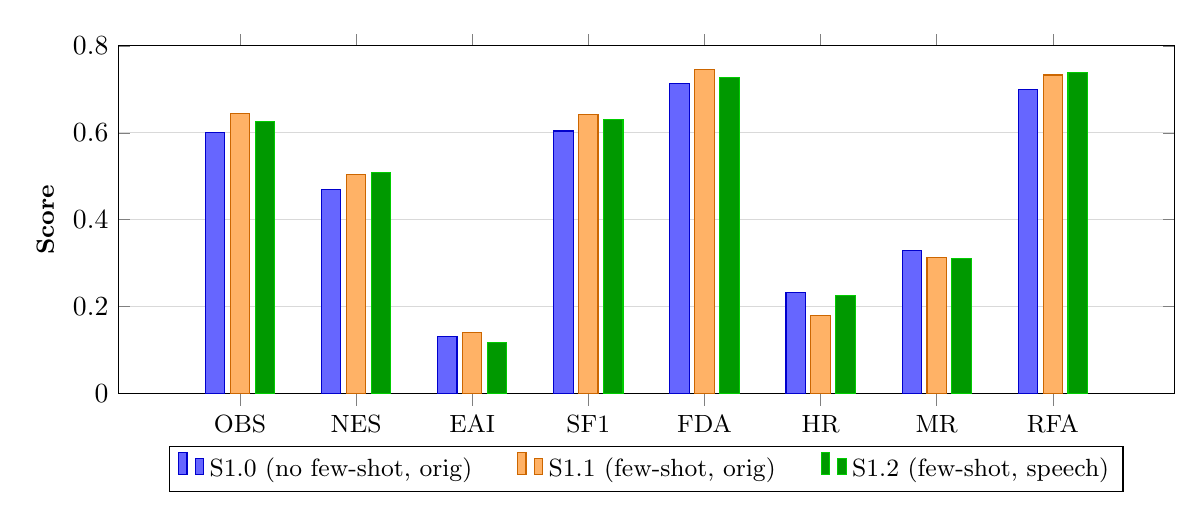
\begin{tikzpicture}
  \begin{axis}[
    width=15cm,
    height=6cm,
    ybar,
    bar width=7pt,
    ylabel={Score},
    ylabel style={font=\small\bfseries},
    xlabel={Metrics},
    xlabel style={font=\small\bfseries},
    symbolic x coords={OBS, NES, EAI, SF1, FDA, HR, MR, RFA},
    xtick=data,
    xticklabel style={font=\small},
    ymin=0,
    ymax=0.8,
    ytick={0, 0.2, 0.4, 0.6, 0.8},
    ymajorgrids=true,
    grid style={line width=0.3pt, draw=gray!30},
    legend style={
      at={(0.5,-0.15)},
      anchor=north,
      legend columns=3,
      font=\small,
      /tikz/every even column/.append style={column sep=0.5cm}
    },
    enlarge x limits=0.15,
  ]
  
  % S1.0 (no few-shot, orig) - Blue
  \addplot[fill=blue!60, draw=blue!80!black] coordinates {
    (OBS, 0.601)
    (NES, 0.469)
    (EAI, 0.132)
    (SF1, 0.604)
    (FDA, 0.713)
    (HR, 0.233)
    (MR, 0.329)
    (RFA, 0.700)
  };
  \addlegendentry{S1.0 (no few-shot, orig)}
  
  % S1.1 (few-shot, orig) - Orange
  \addplot[fill=orange!60, draw=orange!80!black] coordinates {
    (OBS, 0.644)
    (NES, 0.504)
    (EAI, 0.140)
    (SF1, 0.642)
    (FDA, 0.746)
    (HR, 0.180)
    (MR, 0.313)
    (RFA, 0.733)
  };
  \addlegendentry{S1.1 (few-shot, orig)}
  
  % S1.2 (few-shot, speech) - Green
  \addplot[fill=green!60!black, draw=green!80!black] coordinates {
    (OBS, 0.626)
    (NES, 0.508)
    (EAI, 0.118)
    (SF1, 0.631)
    (FDA, 0.727)
    (HR, 0.226)
    (MR, 0.311)
    (RFA, 0.738)
  };
  \addlegendentry{S1.2 (few-shot, speech)}
  
  \end{axis}
\end{tikzpicture}
\caption{Performance of S1 strategy variants on the MUC-4 subset ($N{=}100$). The chart compares zero-shot prompting (S1.0), few-shot prompting on clean text (S1.1), and few-shot prompting on speech-style inputs (S1.2). Few-shot prompting improves key metrics such as OBS, SF1, and FDA while lowering HR and MR, with S1.2 maintaining most benefits despite noisier inputs.}
\label{fig:s1-variants-bar}
\end{figure}

\begin{figure}[H]
\centering
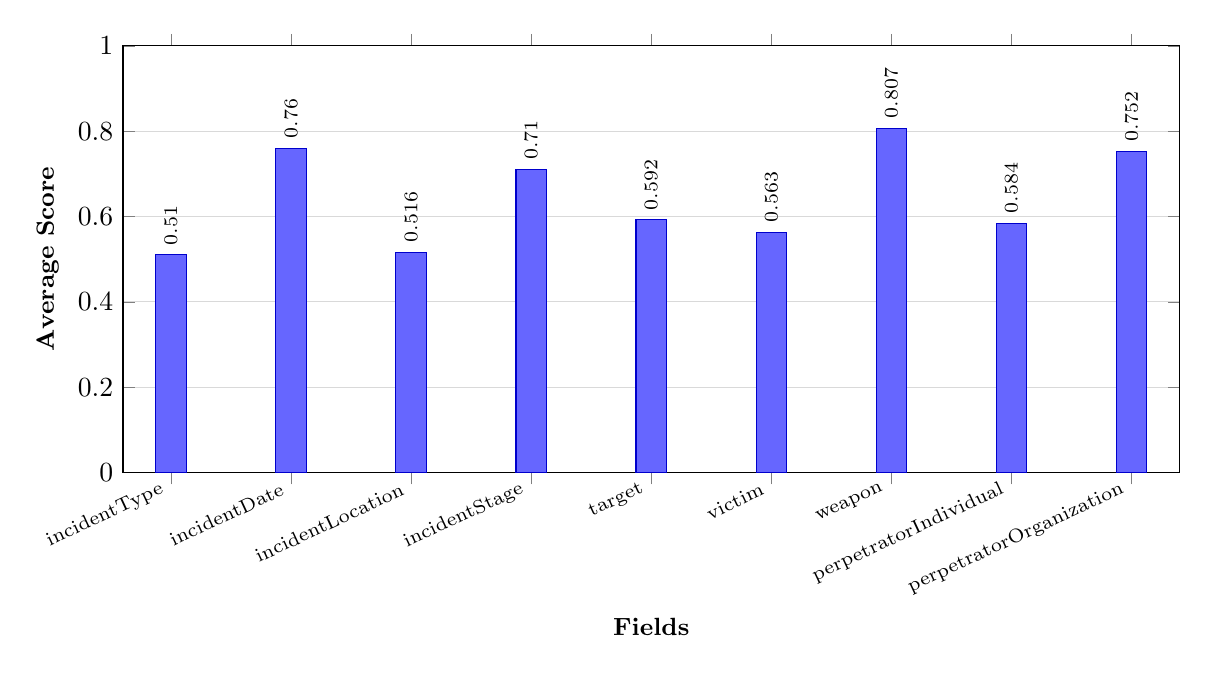
\begin{tikzpicture}
  \begin{axis}[
    width=15cm,
    height=7cm,
    ybar,
    bar width=11pt,
    ylabel={Average Score},
    ylabel style={font=\small\bfseries},
    xlabel={Fields},
    xlabel style={font=\small\bfseries},
    symbolic x coords={
      incidentType,
      incidentDate,
      incidentLocation,
      incidentStage,
      target,
      victim,
      weapon,
      perpetratorIndividual,
      perpetratorOrganization,
    },
    xtick=data,
    xticklabel style={font=\scriptsize, rotate=25, anchor=east},
    ymin=0,
    ymax=1.0,
    ytick={0,0.2,0.4,0.6,0.8,1.0},
    ymajorgrids=true,
    grid style={line width=0.3pt, draw=gray!30},
    enlarge x limits=0.05,
    nodes near coords,
    nodes near coords style={
        font=\scriptsize,
        rotate=90,
        anchor=west,
        /pgf/number format/precision=3
    }
  ]
  
  \addplot[fill=blue!60, draw=blue!80!black] coordinates {
    (incidentType, 0.510)
    (incidentDate, 0.760)
    (incidentLocation, 0.516)
    (incidentStage, 0.710)
    (target, 0.592)
    (victim, 0.563)
    (weapon, 0.807)
    (perpetratorIndividual, 0.584)
    (perpetratorOrganization, 0.752)
  };
  
  \end{axis}
\end{tikzpicture}

\caption{Per-field extraction performance for S1.1 on the MUC-4 subset ($N{=}100$). Structured fields such as \textit{incidentDate} and \textit{weapon} show high accuracy, whereas open-ended categories like \textit{incidentType} and \textit{incidentLocation} remain challenging. The pattern illustrates where few-shot prompting is effective and where additional support mechanisms may be required.}
\label{fig:s1-perfield-plot}
\end{figure}

\paragraph{Per-field behaviour (S1.1).}

\texttt{perpetratorOrganization} and \texttt{weapon} are the strongest fields under S1.1, whereas \texttt{perpetratorIndividual} and \texttt{incidentLocation} remain more challenging.

\subsection*{Latency}

\begin{figure}[H]
\centering
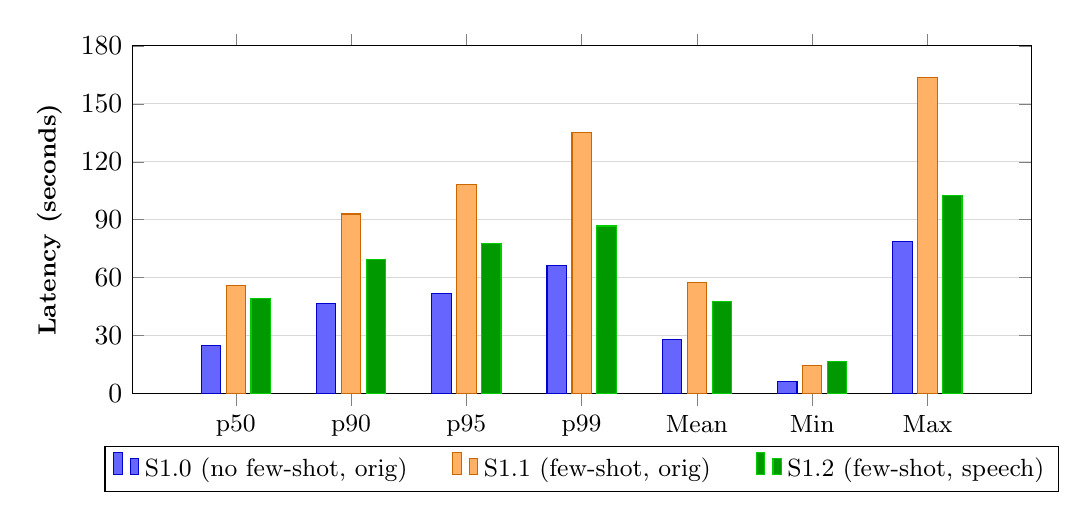
\begin{tikzpicture}
  \begin{axis}[
    width=13cm,
    height=6cm,
    ybar,
    bar width=7pt,
    ylabel={Latency (seconds)},
    ylabel style={font=\small\bfseries},
    xlabel={Statistics},
    xlabel style={font=\small\bfseries},
    symbolic x coords={p50, p90, p95, p99, Mean, Min, Max},
    xtick=data,
    xticklabel style={font=\small},
    ymin=0,
    ymax=180,
    ytick={0, 30, 60, 90, 120, 150, 180},
    ymajorgrids=true,
    grid style={line width=0.3pt, draw=gray!30},
    legend style={
      at={(0.5,-0.15)},
      anchor=north,
      legend columns=3,
      font=\small,
      /tikz/every even column/.append style={column sep=0.5cm}
    },
    enlarge x limits=0.15,
  ]
  
  % S1.0 (no few-shot, orig) - Blue
  \addplot[fill=blue!60, draw=blue!80!black] coordinates {
    (p50, 25.04)
    (p90, 46.49)
    (p95, 51.82)
    (p99, 66.12)
    (Mean, 28.17)
    (Min, 6.51)
    (Max, 78.65)
  };
  \addlegendentry{S1.0 (no few-shot, orig)}
  
  % S1.1 (few-shot, orig) - Orange
  \addplot[fill=orange!60, draw=orange!80!black] coordinates {
    (p50, 55.91)
    (p90, 93.01)
    (p95, 108.40)
    (p99, 134.93)
    (Mean, 57.34)
    (Min, 14.54)
    (Max, 163.79)
  };
  \addlegendentry{S1.1 (few-shot, orig)}
  
  % S1.2 (few-shot, speech) - Green
  \addplot[fill=green!60!black, draw=green!80!black] coordinates {
    (p50, 49.36)
    (p90, 69.30)
    (p95, 77.84)
    (p99, 86.79)
    (Mean, 47.89)
    (Min, 16.85)
    (Max, 102.50)
  };
  \addlegendentry{S1.2 (few-shot, speech)}
  
  \end{axis}
\end{tikzpicture}
\caption{Latency statistics for S1 variants (seconds).}
\label{fig:s1-latency-bar}
\end{figure}

Figure~\ref{fig:s1-perfield-plot} confirms that performance is not uniform across slots. Categorical fields such as \texttt{incidentStage}, \texttt{perpetratorOrganization}, and especially \texttt{weapon} achieve relatively high scores, reflecting their clearer lexical patterns and more constrained label spaces. In contrast, \texttt{perpetratorIndividual} and \texttt{incidentLocation} show lower averages, consistent with their higher ambiguity and sparsity in the underlying texts. Dates are handled comparatively well (average $0.760$ for \texttt{incidentDate}), but the remaining gap to perfect accuracy indicates residual issues with normalization and partial matches.

Figure~\ref{fig:s1-latency-bar} illustrates the latency–quality trade-off within the S1 family. S1.0 is clearly the fastest variant, with a median of around $25$\,s per document and a relatively short tail, but it is also the weakest in terms of accuracy. S1.1 roughly doubles the median latency to about $56$\,s and exhibits a long tail up to approximately $164$\,s, reflecting the additional computation needed to incorporate few-shot context. S1.2 offers an intermediate profile: its median latency ($\sim 49$\,s) and mean latency are lower than S1.1, and the upper tail is substantially shorter (p99 $=86.8$\,s vs.\ $134.9$\,s), making it more attractive in scenarios where robustness to speech-style inputs is required but extreme latency must be avoided.

\subsection*{Cost Analysis (S1: Single-Pass Full Input)}

\textbf{Assumptions.} Extraction uses \textit{GPT-5} with $I{=}3{,}000$ input tokens and $O{=}300$ output tokens; verification uses \textit{GPT-5-mini} with $V_{\text{in}}{=}1{,}000$ and $V_{\text{out}}{=}100$. If audio is present, an additional Whisper transcription cost is incurred for $D$ minutes of audio.

\textbf{Prices.} GPT-5: input \$1.25/M, output \$10.00/M. GPT-5-mini: input \$0.25/M, output \$2.00/M. Whisper: \$0.006/min.

\textbf{Formula.}
\[
\text{Cost}=\frac{I}{10^6}p_{\text{in}}+\frac{O}{10^6}p_{\text{out}}
+\frac{V_{\text{in}}}{10^6}p^{(\text{mini})}_{\text{in}}
+\frac{V_{\text{out}}}{10^6}p^{(\text{mini})}_{\text{out}}
+0.006\cdot D
\]

\textbf{Per-record (no audio).}
\[
\underbrace{\tfrac{3000}{10^6}\!\cdot\!1.25}_{\$0.00375}
+\underbrace{\tfrac{300}{10^6}\!\cdot\!10.00}_{\$0.00300}
+\underbrace{\tfrac{1000}{10^6}\!\cdot\!0.25}_{\$0.00025}
+\underbrace{\tfrac{100}{10^6}\!\cdot\!2.00}_{\$0.00020}
=\mathbf{\$0.00720}\ (\approx 0.72\text{¢/doc})
\]

\textbf{With audio (Whisper).} Adding Whisper introduces a simple linear term $0.006\cdot D$. For $D{=}1$\,min, the total cost becomes $\$0.00720 + 0.006 = \mathbf{\$0.01320}$ (approximately $1.32$\,¢ per document). At the token scales considered here, S1’s LLM component remains inexpensive (around \$0.0072 per document), and audio processing dominates cost for longer recordings.

\subsection*{Consistency (Formatting \& Style)}

Figure~\ref{fig:s1-consistency} shows that few-shot prompting improves both schema-level and style-level consistency. S1.1 achieves the highest schema format preservation ($\mathrm{FPR}_{\text{overall}}{=}0.960$) and the best style consistency score ($\mathrm{SC}_{\text{macro}}{=}0.724$), confirming that the additional examples help the model adhere more reliably to the expected JSON schema and textual conventions. S1.2 remains close to S1.1 despite the more challenging speech-style input, with only a small drop in both scores, which indicates that the single-pass architecture can maintain formatting and stylistic regularity even under noisier conditions.

Taken together, the three S1 variants illustrate how single-pass extraction behaves under different prompting and input conditions. The addition of few-shot examples consistently strengthens the model: S1.1 delivers the highest overall accuracy on clean text, with notable gains in FDA, SF1, and schema–style consistency, albeit at the cost of higher latency. S1.2 provides a balanced alternative for speech-like transcripts, maintaining competitive accuracy while reducing tail latency and showing the strongest behaviour under nonempty–nonempty evaluation (NES, RFA). In contrast, S1.0 represents a minimal baseline without contextual guidance—fastest but clearly weakest across core metrics. Overall, S1.1 is the most effective configuration for high-quality offline extraction, whereas S1.2 is preferable in interactive or speech-driven deployments where robustness and latency stability matter.

\begin{figure}[H]
\centering
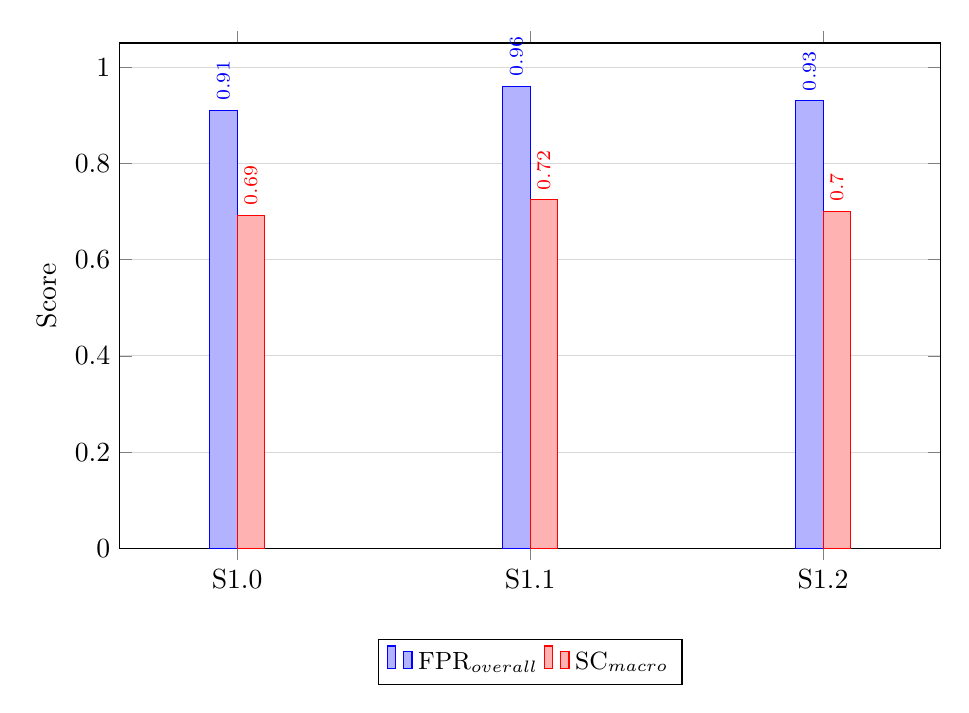
\begin{tikzpicture}
  \begin{axis}[
    width=12cm,
    height=8cm,
    ybar=0pt,
    bar width=10pt,
    ymin=0, ymax=1.05,
    ylabel={Score},
    symbolic x coords={S1.0,S1.1,S1.2},
    xtick=data,
    ymajorgrids=true,
    grid style={line width=0.3pt, draw=gray!30},
    legend style={at={(0.5,-0.18)}, anchor=north, legend columns=2, font=\small},
    enlarge x limits=0.20,
    nodes near coords,
    nodes near coords style={
      font=\scriptsize,
      rotate=90,
      anchor=west,
    },
  ]

    \addplot coordinates {(S1.0,0.910) (S1.1,0.960) (S1.2,0.930)};
    \addlegendentry{$\mathrm{FPR}_{\text{overall}}$}

    \addplot coordinates {(S1.0,0.692) (S1.1,0.724) (S1.2,0.700)};
    \addlegendentry{$\mathrm{SC}_{\text{macro}}$}

  \end{axis}
\end{tikzpicture}
\caption{Consistency (S1 variants): schema formatting vs.\ input-aware style.}
\label{fig:s1-consistency}
\end{figure}

